\section{Related Work}

Before delving into the methods and algorithms developed as part of this thesis, a survey of existing open source navigation packages is neccessary. This will provide background for the design choices in this thesis as deficincies in these existing packages were areas that this thesis focused on improving upon. Specifically, the most mature and complete open source navigation package is that available in the Robot Operating System (ROS)\autocite{Marder-Eppstein2010}; due to this maturity and completeness, the ROS navigation stack will be the primary focus of this examination of related work. The ROS navigation stack is made up into four distinct parts that will be detailed in individual sections: obstacle mapping, local planning, global planning and localization.

\subsection{Obstacle Mapping}

\begin{figure}
\centering
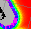
\includegraphics[width=0.75\textwidth]{images/costmap_2d_costgradient}
\caption{costmap\_2d sample \label{fig:costmap_2d_costgradient}}
\end{figure}

For obstacle mapping, the ROS navigation stack uses a software package called "costmap\_2d" \todo{reference to costmap2d wiki page}. This package takes in sensor information about the environment, builds a 2D or 3D fixed-resolution occupancy grid by raytracing that sensor information and inflates obstacles to facilitate navigation based on user provided robot parameters. For a visualization of a small portion of a costmap built from actual sensor data, see \autoref{fig:costmap_2d_costgradient}. In \autoref{fig:costmap_2d_costgradient} black pixels are the actual sensed obstacles, gray pixels are marked as "lethal" cost and the rest are a gradient between high cost in violet and low cost in red. Lethal cells are obstacles that have been inflated according the robot's geometry - specifically these are any cells that if the control point (or origin/center) of the robot were to enter one of these cells it would be in collision with the actual sensed obstacle. Outside of this inflated radius (also known as configuration space \todo{reference to configuration space}), the cost gradient expresses a preference for the path planners to stay away from obstacles unless other factors force the robot near to the obstacle.

While this approach works in many environments, it has drawbacks when used for precision navigation. The most serious drawback is the fixed resolution of the grid when very fine resolution is required for some areas, but not others. For example, imagine navigating through a narrow doorway that opens to wide open areas on either side. In this situation, there is generally no good overall choice for the resolution of the grid. Choosing a resolution that is fine enough to ensure that the robot can always fit through the doorway leads to an unnecessarily large number of empty cells in the wide open areas, wasting both memory and computation time evaluating these cells; choosing a resolution that reduces the number of cells in the open areas may not guarantee that the doorway will always be sensed as traversable, as even a sensor reading along an edge of a cell will cause the entire cell to be marked as an obstacle. While prior knowledge about an environment allows one to choose a good resolution for that environment, that choice may not be optimal for a different environment; even if an "adaptive" fixed resolution were used that was always optimal for representing a given environment, path planning performance, both how long it takes to find an optimal plan and the actual optimal plan generated, can be affected by changing the obstacle map resolution, which is undesirable for a navigation system that seeks to perform consistently in different environments.

Another issue with the implementation used by costmap\_2d is that, with a very fine grid cell resolution, obstacles can leave "droppings" in the map. These "droppings" occur when an obstacle such as a human moves across the sensor's field of view and is not completely cleared out of the map because raytracing the sensor beams does not intersect all of the cells that the obstacle had already marked as occupied. In order to resolve this problem, either a large enough grid cell resolution must be used to ensure that sensor beams will never fall to either side of an occupied cell (but, as discussed previously, large grid cell resolutions have other significant drawbacks) or an occupancy grid implementation that can clear cells even if a sensor beam does not raytrace through a particular cell must be used. For example, an occupancy grid implementation could slowly "fade" obstacle cells so that obstacles that have not been observed for some time would automatically be cleared. Other possibilities include explicitly modeling the probability of each cell given all of the previous sensor measurements, such as the occupancy grid mappying techniques introduced in \autocite{Moravec_1985_1840}. The proposed mapping solution used in this thesis is detailed in \todo{reference section where I talk about octocostmap and costmap3d}.

\subsection{Local Planning}

Base Local Planner

\begin{comment}
This will detail problems in ROS's Navigation stack when we last looked at it (and perhaps a discussion of how it has changed in the interim)

Outline:
	Mapping
		SimpleCostmap
		Fixed Grid size - needs changed for different environments and may affect trajectory scoring
		No option for temporal clearing of the map to reduce "leftovers" at small resolutions
	Local planning
		Scoring of trajectories
		Trajectories come from a fixed list of velocities and omegas (cross-product)
		simplistic cost function
		holonomic vs diff-drive
		scoring spin-in-place
	global planning
		dijkstra's planning
		replan only as a last resort
		may generate crappy plan since uses a circular robot with either inscribed or circumscribed radius
	localization
		defaults require tweaking for both map building and amcl
		amcl needs tuned to prevent "pops"
		
\end{comment}
